% Task 2 – Mô hình hóa hệ thống
% Nguồn: docs/diagrams/*.puml, docs/diagrams/README.md
\section{Task 2 -- Mô hình hóa hệ thống}\label{sec:modeling}

Task 2 mô hình hóa hành vi và cấu trúc của BrewLite từ đặc tả ở Task 1. Mọi sơ đồ được viết bằng PlantUML; tệp nguồn
\code{.puml} và ảnh \code{.svg} nằm trong \code{docs/diagrams/}. Mã sơ đồ dùng trong ma trận truy vết:

\begin{table}[H]
\centering
\caption{Danh sách sơ đồ Task 2}\label{tab:diagrams}
\begin{tabularx}{\textwidth}{|l|c|X|l|}
\hline
\thead \textbf{Mã} & \textbf{Task} & \textbf{Nội dung} & \textbf{Tệp nguồn} \\ \hline
Activity-01 & 2.1 & Luồng end-to-end: Xem menu $\rightarrow$ Theo dõi đơn, có swimlane & \code{activity-order-e2e.puml} \\ \hline
Sequence-01 & 2.2 & UC-01 Đặt và thanh toán đơn hàng & \code{sequence-checkout.puml} \\ \hline
Class-01 & 2.3 & Mô hình domain & \code{class-domain.puml} \\ \hline
State-01 & bổ trợ & Vòng đời Order và Payment & \code{state-order-payment.puml} \\ \hline
\end{tabularx}
\end{table}

%%%%%%%%%%%%%%%%%%%%%%%%%%%%%%%%%%%%%%%%%%%%%%%%%%%%%%%%%%%%%%%%%%%%%%
\subsection{Task 2.1 -- Activity diagram}

Sơ đồ Activity-01 mô tả toàn bộ luồng nghiệp vụ tối thiểu của đề bài
(\textit{Xem menu $\rightarrow$ Chọn tùy chọn $\rightarrow$ Giỏ hàng $\rightarrow$ Đặt đơn $\rightarrow$ Thanh toán
$\rightarrow$ Theo dõi đơn}) qua 5 swimlane: hai làn người dùng (Khách hàng, Nhân viên quầy) và ba làn hệ thống
(Next.js UI, NestJS API, Payment Service).

\begin{figure}[H]
\centering
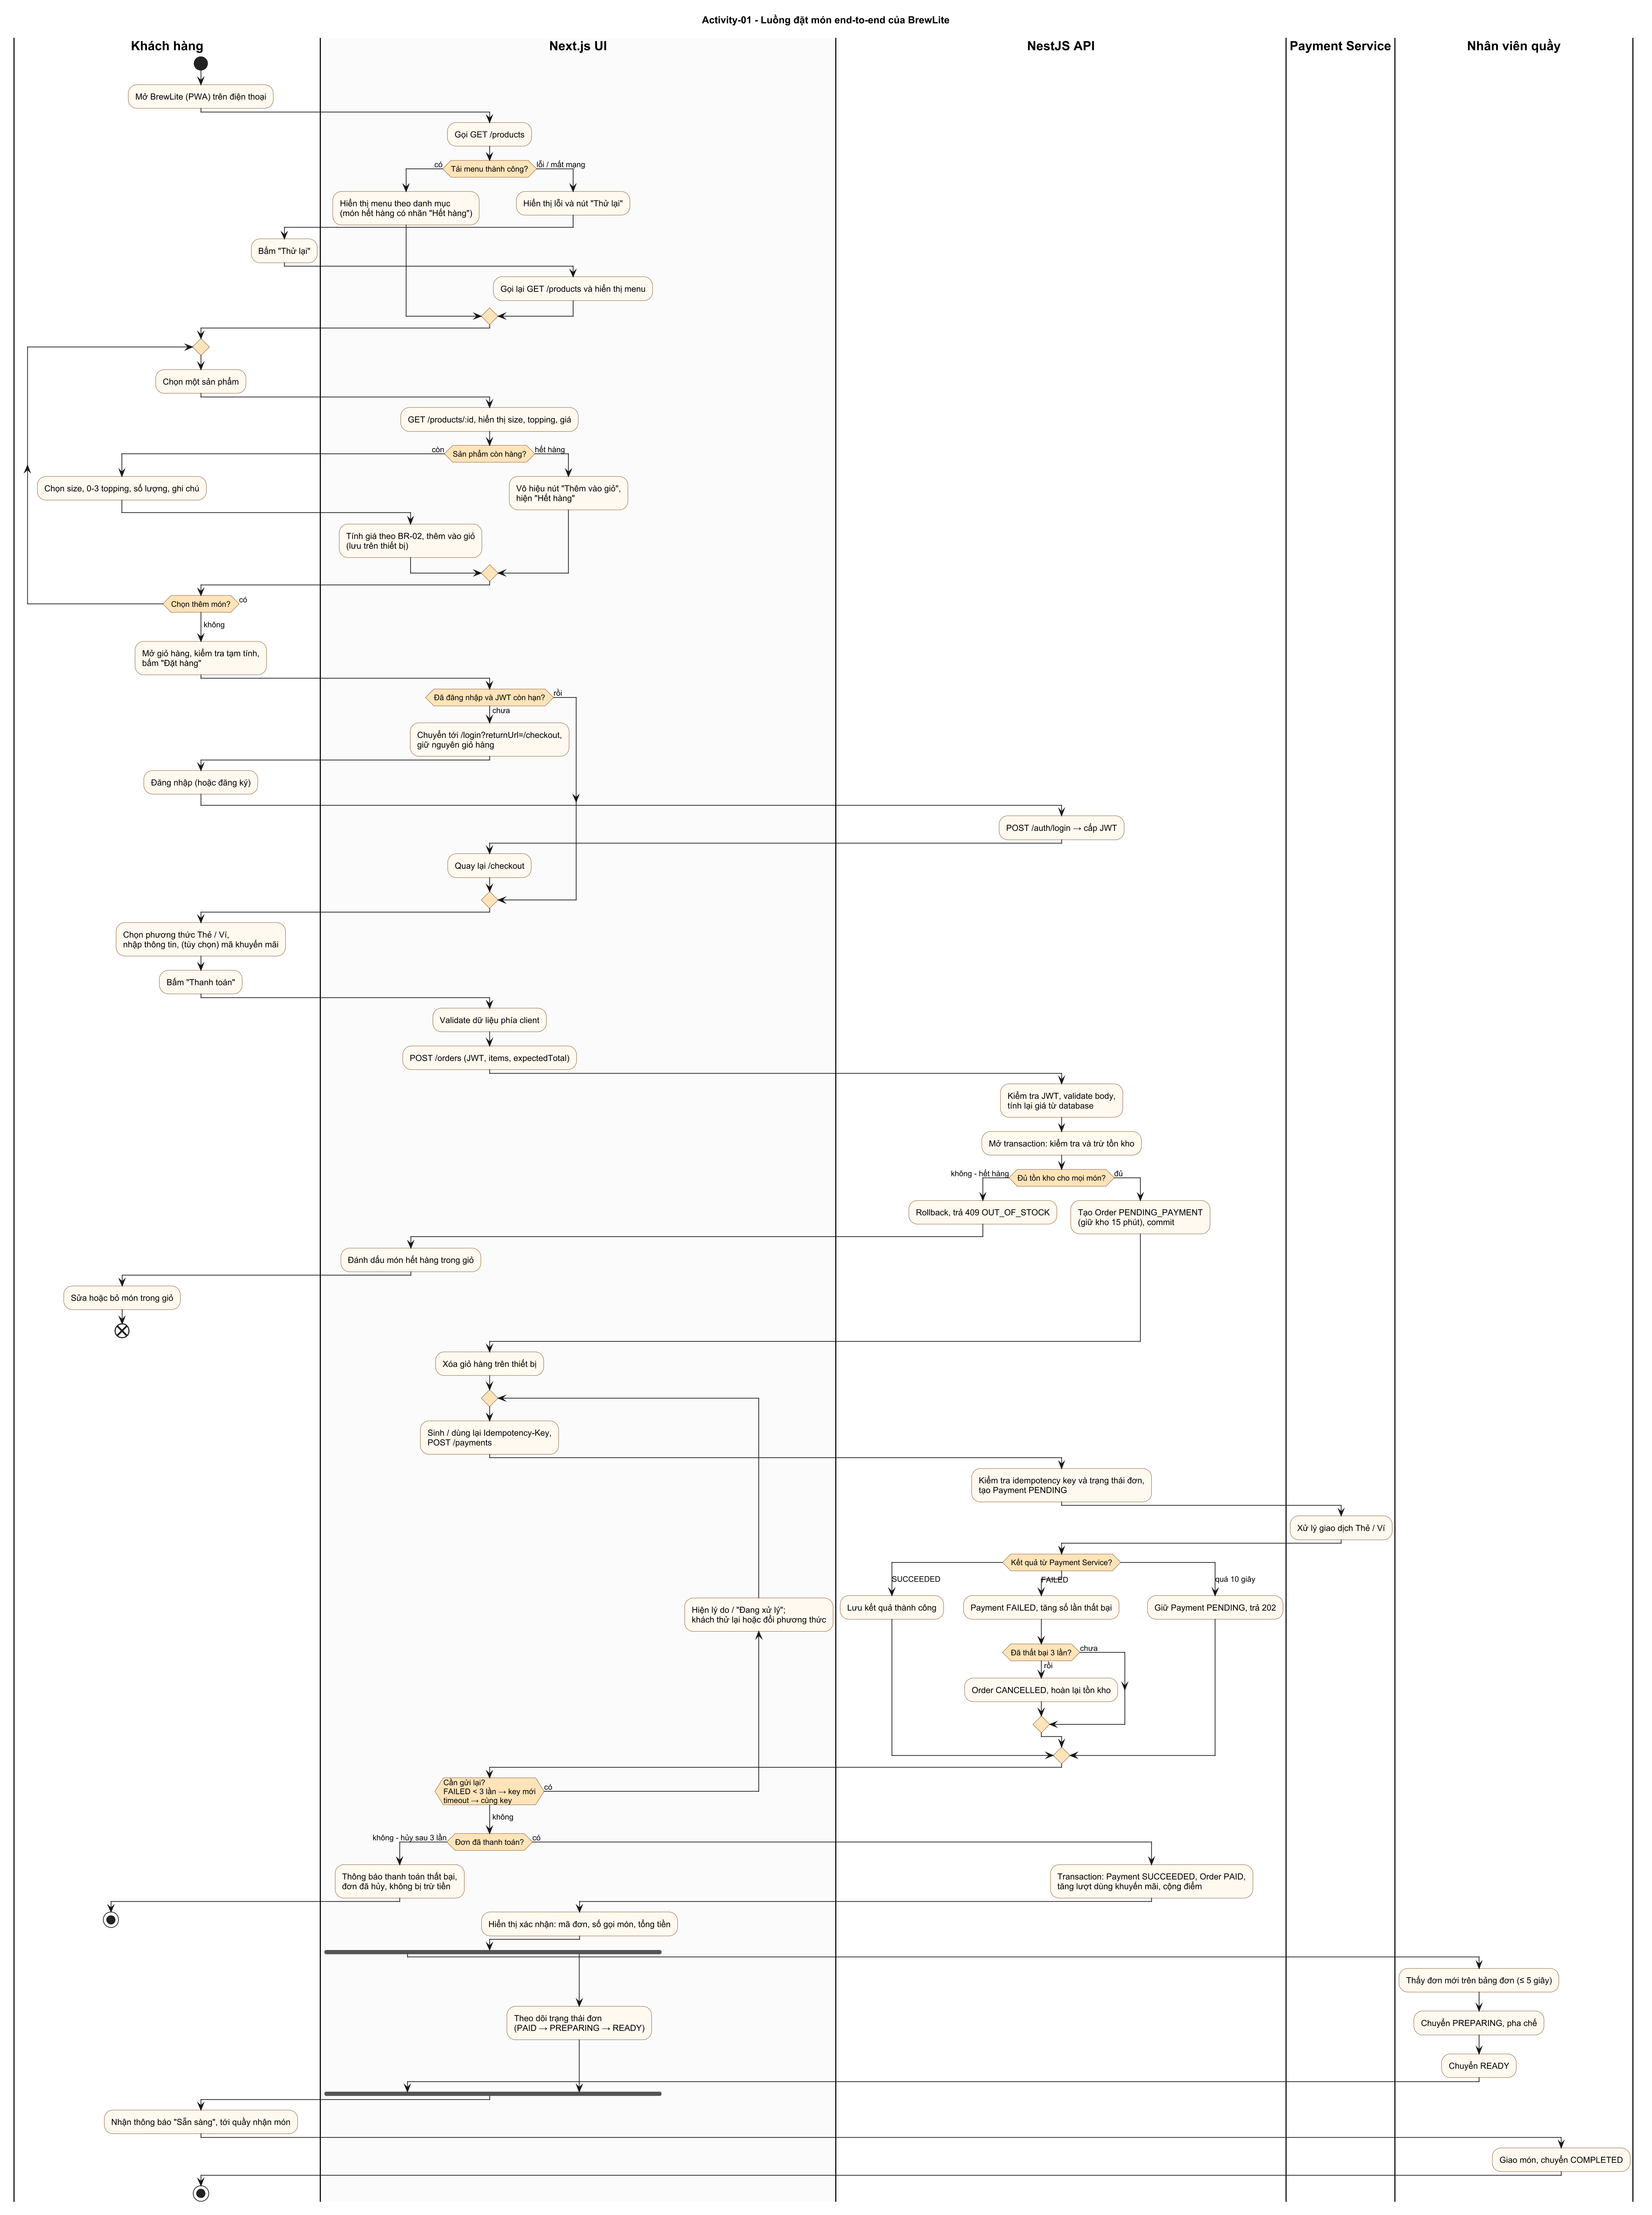
\includegraphics[width=\textwidth,height=0.86\textheight,keepaspectratio]{figures/activity-order-e2e.png}
\caption{Activity-01 -- Luồng đặt món end-to-end (swimlane)}\label{fig:activity}
\end{figure}

\begin{longtable}{|p{3.6cm}|p{11.2cm}|}
\caption{Activity-01 đối chiếu yêu cầu đề bài}\label{tab:activity-check}\\
\hline
\thead \textbf{Yêu cầu của đề} & \textbf{Thể hiện trong sơ đồ} \\ \hline
\endfirsthead
\hline
\thead \textbf{Yêu cầu của đề} & \textbf{Thể hiện trong sơ đồ} \\ \hline
\endhead
Điểm bắt đầu, kết thúc & 1 điểm bắt đầu; 2 điểm kết thúc (đơn hoàn tất; đơn bị hủy sau 3 lần thất bại); 1 flow-final (dừng vì hết hàng, khách quay lại sửa giỏ). \\ \hline
Hành động người dùng và hệ thống & Làn Khách hàng, Nhân viên quầy (người dùng); Next.js UI, NestJS API, Payment Service (hệ thống). \\ \hline
Decision / merge & Tải menu thành công?; Còn hàng?; Chọn thêm món?; Đã đăng nhập?; Đủ tồn kho?; Kết quả thanh toán (3 nhánh); Đã thất bại 3 lần?; Cần gửi lại?; Đơn đã thanh toán? \\ \hline
Swimlane & 5 làn như trên. \\ \hline
Hết hàng & Hai chỗ: ở màn chi tiết sản phẩm (không cho thêm vào giỏ, AC-01.4) và khi tạo đơn (rollback, 409 \code{OUT\_OF\_STOCK}, BR-07). \\ \hline
Chưa đăng nhập & Chuyển \code{/login?returnUrl=/checkout}, giữ giỏ hàng, quay lại thanh toán sau khi đăng nhập (A1, AC-04.1). \\ \hline
Thanh toán thất bại & \code{FAILED}: thử lại bằng key mới; lần thứ 3 thì hủy đơn và hoàn kho (A4, E6, BR-09). Timeout: gửi lại cùng key (A5). \\ \hline
\end{longtable}

%%%%%%%%%%%%%%%%%%%%%%%%%%%%%%%%%%%%%%%%%%%%%%%%%%%%%%%%%%%%%%%%%%%%%%
\newpage
\subsection{Task 2.2 -- Sequence diagram}

Sequence-01 hiện thực use-case trọng tâm UC-01 với đủ 5 lifeline theo đề:
\textit{Customer $\rightarrow$ Next.js UI $\rightarrow$ NestJS API $\rightarrow$ Database $\rightarrow$ Payment Service}.
Sơ đồ chia ba giai đoạn: tạo đơn (\code{POST /orders}), thanh toán (\code{POST /payments}) và thông báo kết quả
cuối cùng (\code{GET /orders/:id}). Bản SVG đầy đủ độ phân giải nằm tại \code{docs/diagrams/sequence-checkout.svg}.

\begin{figure}[H]
\centering
\adjustimage{trim=0 {0.628\height} 0 0,clip,width=\textwidth,height=0.8\textheight,keepaspectratio}{figures/sequence-checkout.png}
\caption{Sequence-01 (phần 1/2) -- Giai đoạn 1: tạo đơn, kiểm tra JWT, validate, transaction trừ kho}\label{fig:sequence}
\end{figure}

\begin{figure}[H]
\centering
\adjustimage{trim=0 0 0 {0.372\height},clip,width=\textwidth,height=0.86\textheight,keepaspectratio}{figures/sequence-checkout.png}
\caption{Sequence-01 (phần 2/2) -- Giai đoạn 2--3: thanh toán, idempotency, \code{alt} thành công/thất bại/timeout, thông báo kết quả}\label{fig:sequence2}
\end{figure}

\begin{longtable}{|p{4.0cm}|p{10.8cm}|}
\caption{Sequence-01 đối chiếu yêu cầu đề bài}\label{tab:sequence-check}\\
\hline
\thead \textbf{Yêu cầu của đề} & \textbf{Thể hiện trong sơ đồ} \\ \hline
\endfirsthead
\hline
\thead \textbf{Yêu cầu của đề} & \textbf{Thể hiện trong sơ đồ} \\ \hline
\endhead
Request/response, thứ tự gọi API & \code{POST /orders} (bước 2--22) $\rightarrow$ \code{POST /payments} (từ bước 26) $\rightarrow$ \code{GET /orders/:id} (giai đoạn 3). \\ \hline
Kiểm tra JWT và validate & \code{JwtAuthGuard} (bước 3, nhánh 401); \code{ValidationPipe} (bước 6, nhánh 400); lặp lại ở \code{POST /payments}. \\ \hline
Transaction tạo đơn và cập nhật tồn kho & Khối \textit{Transaction -- tạo đơn và cập nhật tồn kho}: \code{UPDATE products SET stock = stock - qty WHERE stock >= qty}; không đủ thì \code{ROLLBACK} và 409. \\ \hline
\code{alt} thành công / thất bại & \code{alt} \textit{Thanh toán thành công} / \textit{thất bại} / \textit{timeout 10 giây}. Thành công và thất bại đều được ghi trong transaction. \\ \hline
Idempotency khi gửi lại & \code{alt} \textit{Đã có bản ghi K1}: trả lại response cũ (không gọi Payment Service); 409 khi đang xử lý; 422 khi khác body; gọi lại cổng cùng khóa sau timeout. Bản ghi mới được chèn với ràng buộc \code{UNIQUE(user\_id, key)} để chặn hai request đồng thời. \\ \hline
Thông báo kết quả cuối & ``Thanh toán thành công'' kèm mã đơn, số gọi món, điểm tích được; hoặc lý do thất bại; giai đoạn 3 hiển thị dòng thời gian trạng thái. \\ \hline
\end{longtable}

%%%%%%%%%%%%%%%%%%%%%%%%%%%%%%%%%%%%%%%%%%%%%%%%%%%%%%%%%%%%%%%%%%%%%%
\newpage
\subsection{Task 2.3 -- Class diagram}

Class-01 là mô hình domain gồm 7 lớp bắt buộc (User, Product, Order, OrderItem, Payment, Promotion,
LoyaltyTransaction) và 6 lớp bổ trợ cần để khớp với SRS: Category, ProductSize, Topping, OrderItemTopping,
OrderStatusHistory, IdempotencyRecord.

\begin{figure}[H]
\centering
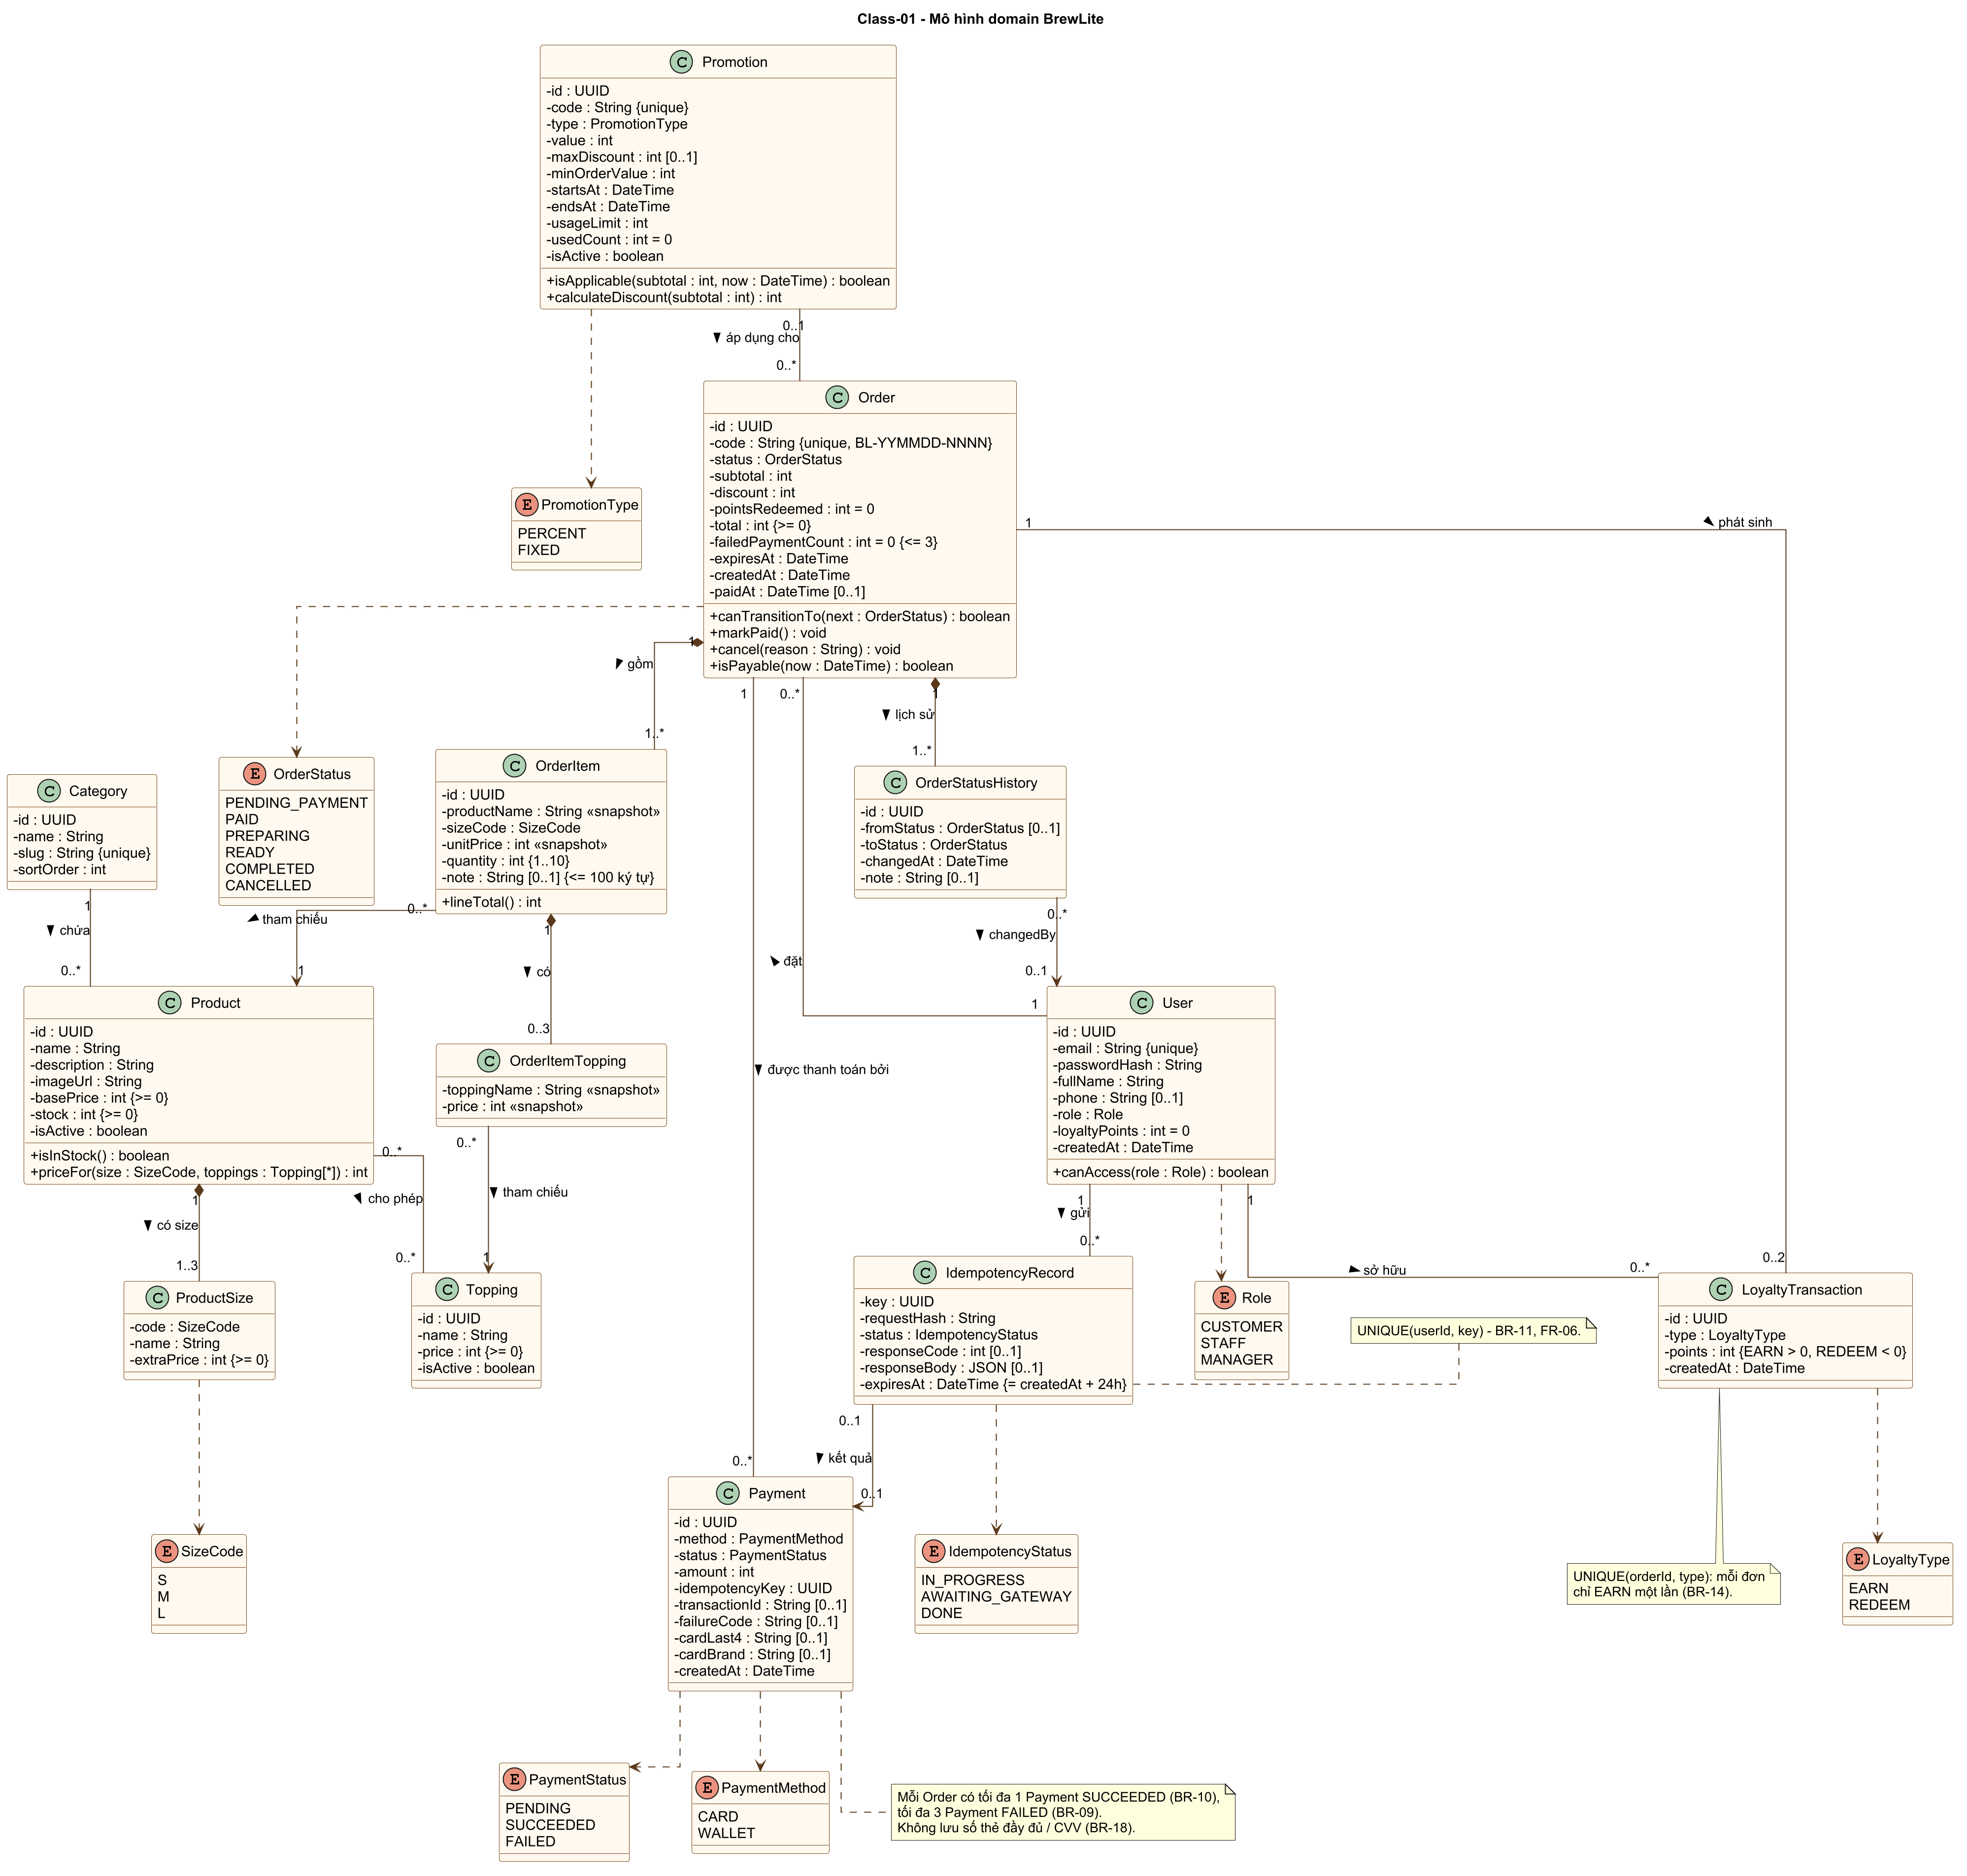
\includegraphics[width=\textwidth,height=0.8\textheight,keepaspectratio]{figures/class-domain.png}
\caption{Class-01 -- Mô hình domain BrewLite}\label{fig:class}
\end{figure}

\begin{longtable}{|p{3.4cm}|p{6.6cm}|p{4.6cm}|}
\caption{Các lớp domain}\label{tab:classes}\\
\hline
\thead \textbf{Lớp} & \textbf{Vai trò và ràng buộc chính} & \textbf{Truy vết} \\ \hline
\endfirsthead
\hline
\thead \textbf{Lớp} & \textbf{Vai trò và ràng buộc chính} & \textbf{Truy vết} \\ \hline
\endhead
User & Tài khoản; \code{email} unique; \code{role}; \code{loyaltyPoints} & FR-09, FR-10, FR-11 \\ \hline
Product & Sản phẩm; \code{basePrice}, \code{stock} $\ge$ 0; \code{isActive} (xóa mềm) & FR-01, FR-02, FR-16, BR-07 \\ \hline
Order & Đơn hàng; mã \code{BL-YYMMDD-NNNN}; \code{expiresAt}; \code{failedPaymentCount} $\le$ 3 & FR-04, BR-08, BR-09, BR-16 \\ \hline
OrderItem & Dòng đơn; snapshot tên và đơn giá; số lượng 1--10 & BR-03, BR-06 \\ \hline
Payment & Một lần thử thanh toán; chỉ lưu \code{cardLast4}; tối đa 1 \code{SUCCEEDED} mỗi đơn & FR-05, BR-10, BR-18 \\ \hline
Promotion & Mã giảm giá \code{PERCENT}/\code{FIXED}, trần, thời hạn, lượt dùng & FR-14, BR-13 \\ \hline
LoyaltyTransaction & Cộng/trừ điểm; \code{UNIQUE(orderId, type)} & FR-15, FR-18, BR-14 \\ \hline
Category & Danh mục menu, \code{slug} unique & FR-17 \\ \hline
ProductSize & Size S/M/L kèm phụ thu & BR-01 \\ \hline
Topping & Topping kèm giá & BR-01, BR-03 \\ \hline
OrderItemTopping & Snapshot topping đã chọn (0--3 mỗi dòng) & BR-03, BR-06 \\ \hline
OrderStatusHistory & Lịch sử chuyển trạng thái, người thực hiện & AC-07.4, AC-12.4 \\ \hline
IdempotencyRecord & Kết quả đã lưu theo khóa; \code{UNIQUE(userId, key)}; hết hạn 24 giờ & FR-06, BR-11 \\ \hline
\end{longtable}

\begin{table}[H]
\centering
\caption{Enum trạng thái}\label{tab:enums}
\begin{tabularx}{\textwidth}{|l|X|l|}
\hline
\thead \textbf{Enum} & \textbf{Giá trị} & \textbf{Truy vết} \\ \hline
OrderStatus & \code{PENDING\_PAYMENT}, \code{PAID}, \code{PREPARING}, \code{READY}, \code{COMPLETED}, \code{CANCELLED} & BR-12 \\ \hline
PaymentStatus & \code{PENDING}, \code{SUCCEEDED}, \code{FAILED} & FR-05 \\ \hline
PaymentMethod & \code{CARD}, \code{WALLET} & FR-05 \\ \hline
PromotionType & \code{PERCENT}, \code{FIXED} & BR-13 \\ \hline
LoyaltyType & \code{EARN}, \code{REDEEM} & BR-14, BR-15 \\ \hline
Role & \code{CUSTOMER}, \code{STAFF}, \code{MANAGER} & FR-11 \\ \hline
SizeCode & \code{S}, \code{M}, \code{L} & BR-01 \\ \hline
IdempotencyStatus & \code{IN\_PROGRESS}, \code{AWAITING\_GATEWAY}, \code{DONE} & FR-06 \\ \hline
\end{tabularx}
\end{table}

\subsection{Sơ đồ trạng thái bổ trợ}
State-01 cố định vòng đời Order và Payment, để ba sơ đồ trên dùng chung một định nghĩa trạng thái.

\begin{figure}[H]
\centering
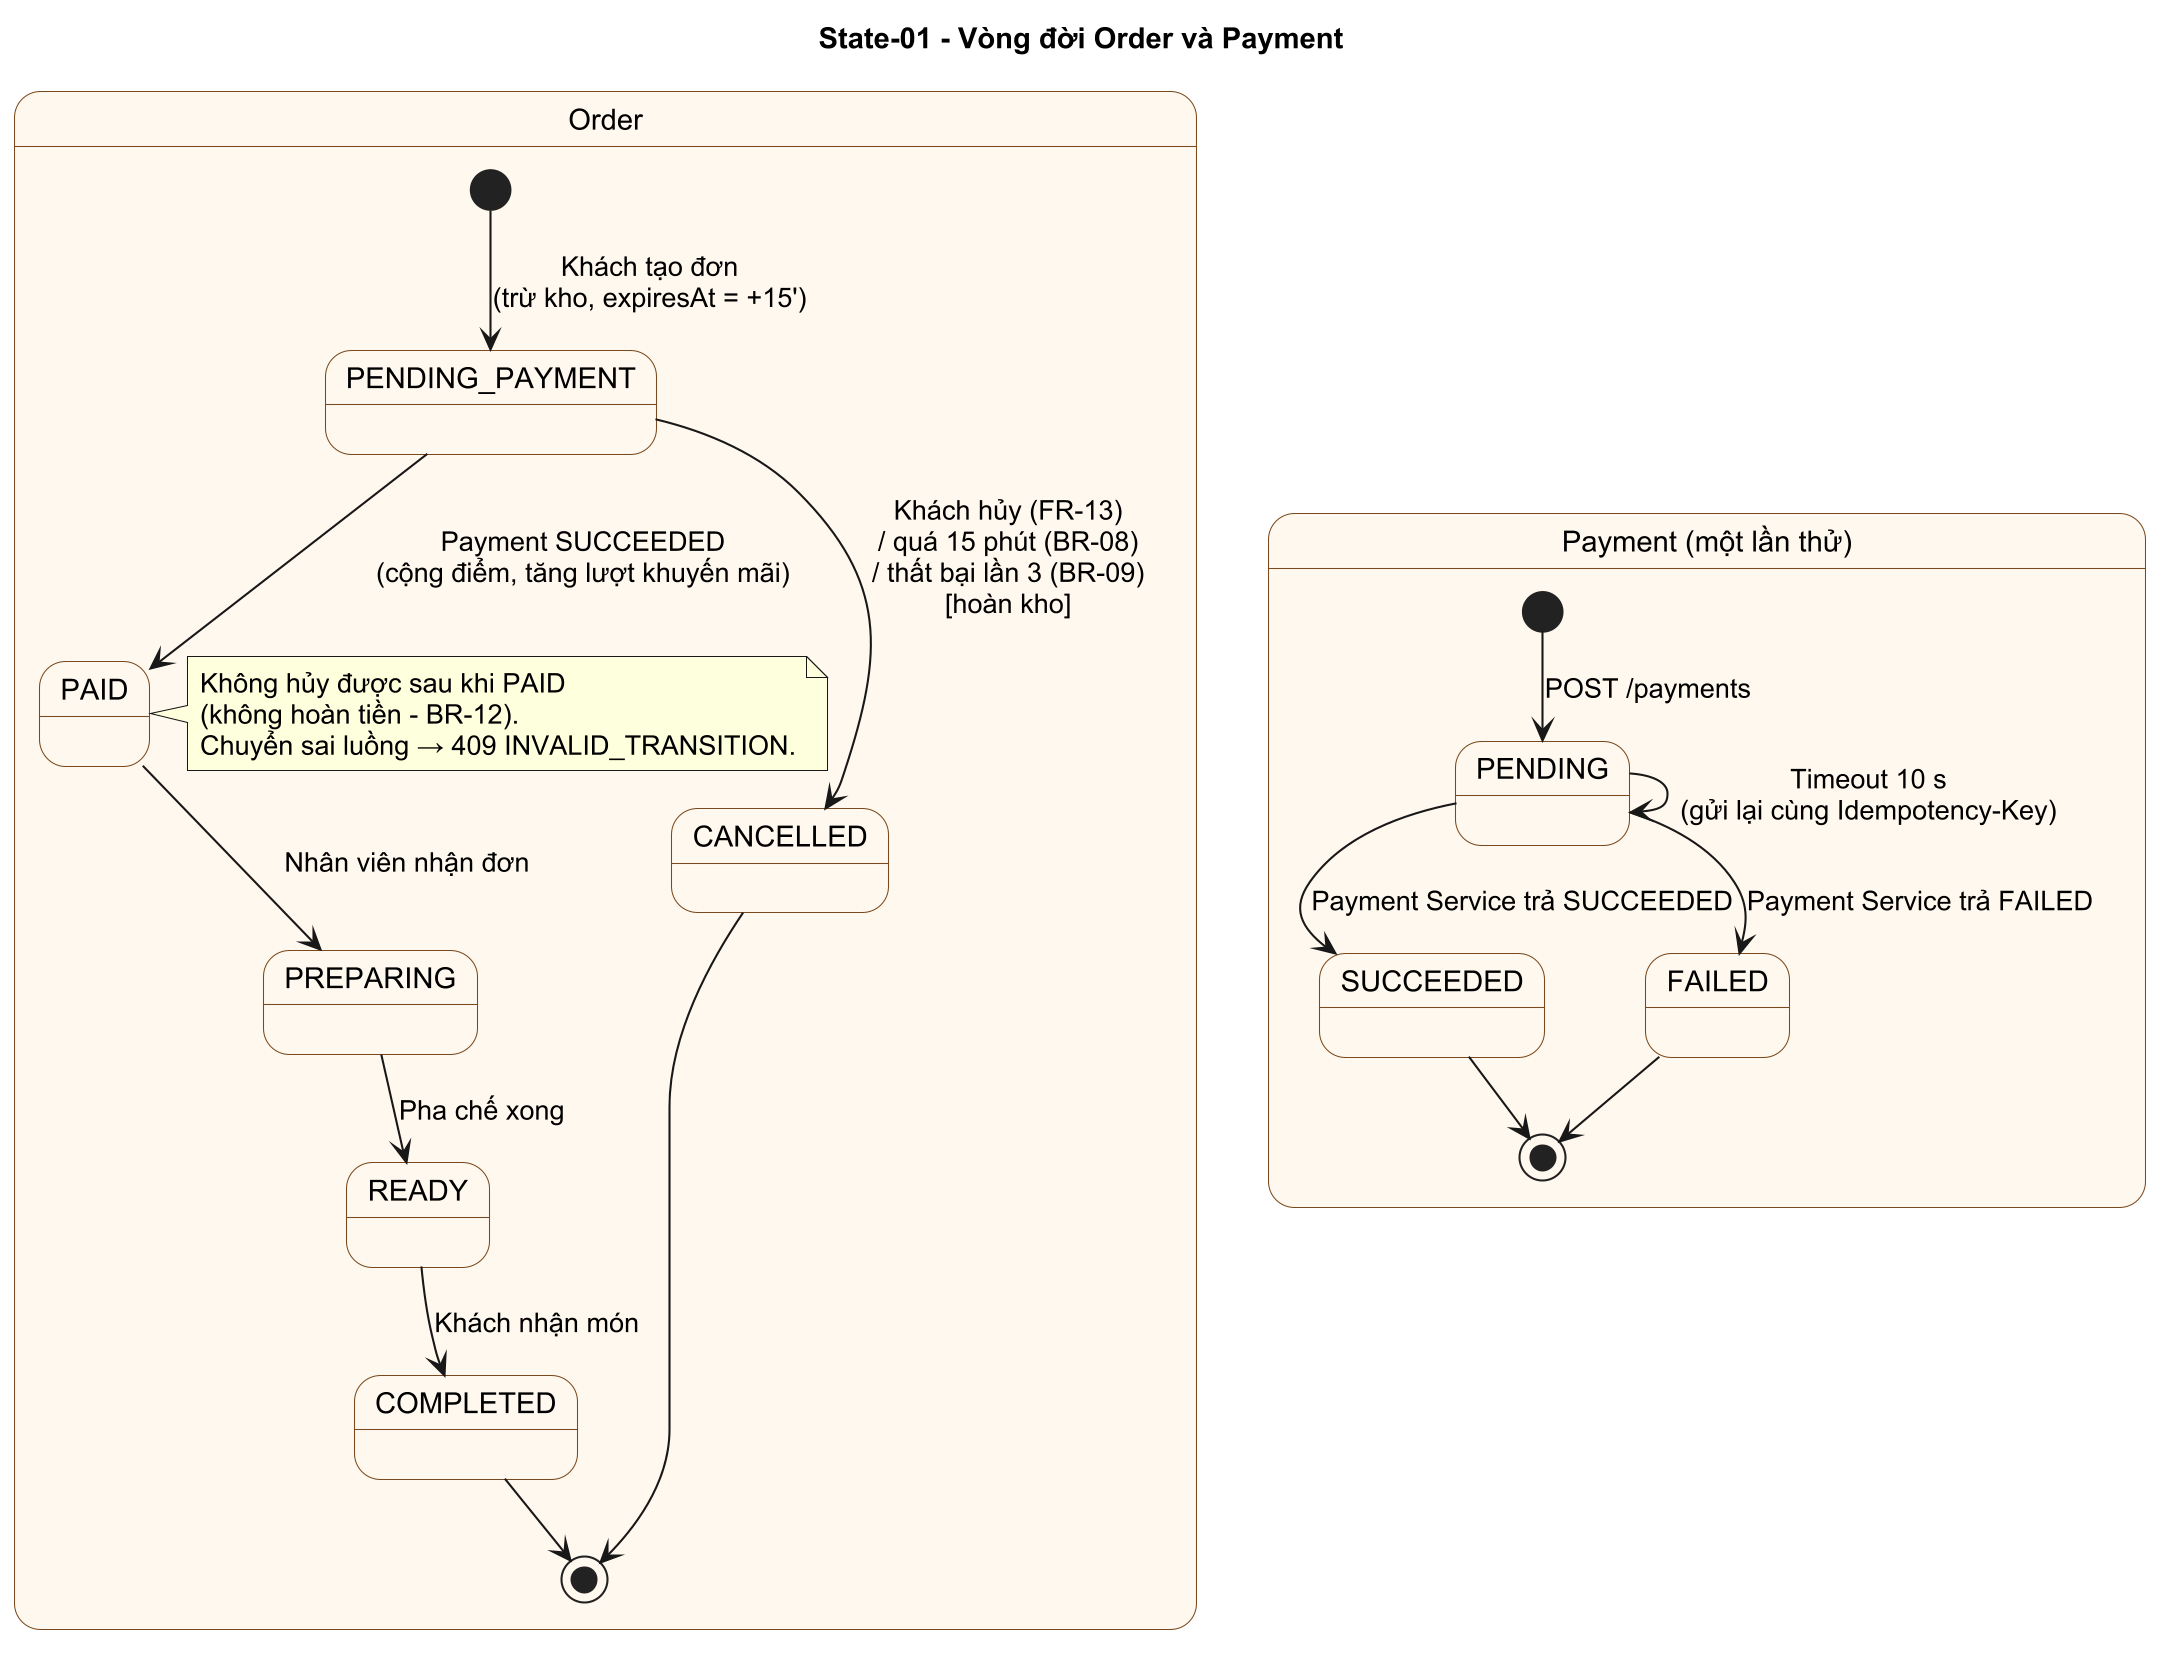
\includegraphics[width=0.9\textwidth]{figures/state-order-payment.png}
\caption{State-01 -- Vòng đời Order và Payment}\label{fig:state}
\end{figure}

%%%%%%%%%%%%%%%%%%%%%%%%%%%%%%%%%%%%%%%%%%%%%%%%%%%%%%%%%%%%%%%%%%%%%%
\subsection{Kiểm tra nhất quán với SRS và use-case}

Tiêu chí nghiệm thu Task 2: \textit{ba loại sơ đồ không mâu thuẫn với SRS, use-case hoặc mô hình dữ liệu.}

{\footnotesize
\begin{longtable}{|p{2.2cm}|p{2.4cm}|p{2.7cm}|p{3.4cm}|p{3.4cm}|}
\caption{Đối chiếu nhất quán giữa các sơ đồ và SRS}\label{tab:consistency}\\
\hline
\thead \textbf{Khái niệm} & \textbf{SRS / Use-case} & \textbf{Activity-01} & \textbf{Sequence-01} & \textbf{Class-01 / State-01} \\ \hline
\endfirsthead
\hline
\thead \textbf{Khái niệm} & \textbf{SRS / Use-case} & \textbf{Activity-01} & \textbf{Sequence-01} & \textbf{Class-01 / State-01} \\ \hline
\endhead
Trạng thái đơn & BR-12 & Đúng thứ tự, nhân viên đổi trạng thái & \code{PENDING\_PAYMENT} $\rightarrow$ \code{PAID}; \code{CANCELLED} sau 3 lần & \code{OrderStatus} 6 giá trị; 7 chuyển trạng thái \\ \hline
Trạng thái thanh toán & AC-05.4 $\rightarrow$ 05.7 & Switch 3 nhánh & \code{alt} 3 nhánh & \code{PaymentStatus} 3 giá trị \\ \hline
Trừ kho & BR-07 & Transaction trừ kho & \code{UPDATE ... stock >= qty} & \code{stock} $\ge$ 0 \\ \hline
Giữ kho 15 phút & BR-08 & ``giữ kho 15 phút'' & \code{expires\_at = now + 15'} & \code{Order.expiresAt} \\ \hline
Tối đa 3 lần thất bại & BR-09 & ``Đã thất bại 3 lần?'' & \code{opt} count = 3 & \code{failedPaymentCount} $\le$ 3 \\ \hline
Idempotency & BR-11, FR-06 & Sinh / dùng lại key & \code{alt} đã có K1 & \code{IdempotencyRecord} \\ \hline
Khuyến mãi & BR-13, FR-14 & Nhập mã khi thanh toán & \code{used\_count + 1} khi PAID & \code{Promotion.usedCount} \\ \hline
Tích điểm & BR-14, FR-15 & Cộng điểm khi PAID & \code{INSERT loyalty\_transactions} & \code{UNIQUE(orderId, type)} \\ \hline
Snapshot giá & BR-06 & -- & snapshot trong \code{order\_items} & \code{<<snapshot>>} \\ \hline
Không lưu số thẻ & BR-18 & -- & \code{card\_last4} & Chỉ có \code{cardLast4} \\ \hline
Bắt buộc đăng nhập & A6, AC-04.1 & Nhánh chưa đăng nhập & Nhánh 401 & \code{User.role} \\ \hline
\end{longtable}
}
